\item \points{25} {\bf Learning Imbalanced dataset}

In this problem, we study how to learn a classifier from an imbalanced dataset, where the marginal distribution of the classes/labels are imbalanced. Imbalanced datasets are ubiquitous in real-world applications. For example, in the spam detection problem, the training dataset usually has only a small fraction of spam emails (positive examples) but a large fraction of ordinary emails (negative examples). For simplicity, we consider binary classification problem where the labels are in $\{0,1\}$ and the number of positive examples is much smaller than the number of negative examples. 


\begin{enumerate}
        \item \subquestionpoints{10} \textbf{Evaluation metrics}

In this sub-question, we discuss the common evaluation metrics for imbalanced dataset. Suppose we have a validation dataset and for some $\rho \in (0,1)$, we assume that $\rho$ fraction of the validation examples are positive examples (with label 1), and $1-\rho$ fraction of them are negative examples (with label 0). 


Define the accuracy as
\begin{align*}
A \triangleq %\frac{TN+TN}{TP+TN + FP+FN} 
\frac{\# \textrm{examples that are predicted correctly by the classifier}}{\# \textrm{examples}} 
\end{align*}
(i) (3 point) Show that for any dataset with $\rho$ fraction of positive examples and $1-\rho$ fraction of negative examples, there exists a (trivial) classifier with accuracy at least $1-\rho$. 
\newline
\\
The statement above suggests that the accuracy is not an ideal evaluation metric when $\rho$ is close to 0. E.g., imagine that for spam detection $\rho$ can be smaller than 1\%. The statement suggests there is a trivial classifier that gets more than 99\% accuracy. This could be misleading ---  99\% seems to be almost perfect, but actually you don't need to learn anything from the dataset to achieve it. 

Therefore, for imbalanced dataset, we need more informative evaluation metrics. We define the number of true positive, true negative, false positive, false negative examples as
\begin{align*}
TP & \triangleq \# \textrm{ positive examples with a correct (positive) prediction} \\
TN & \triangleq \# \textrm{ negative examples with a correct (negative) prediction} \\
FP & \triangleq \# \textrm{ negative examples with a incorrect (positive) prediction} \\
FN & \triangleq \# \textrm{ positive examples with a incorrect (negative) prediction} 
\end{align*}

Define the accuracy of positive examples  as 
\newcommand{\recall}{\textup{recall}}
\begin{align*}
A_1 &\triangleq \frac{TP}{TP + FN} = \frac{\#  \textrm{ positive examples with a correct (positive) prediction}}{\# \textrm{ positive examples}}\nonumber\\
\end{align*}
Define the accuracy of negative examples as 
\begin{align*}
A_0 & \triangleq \frac{TN}{TN + FP} = \frac{\#  \textrm{ negative examples with a correct (negative) prediction}}{\# \textrm{ negative examples}}
\end{align*}

We define the balanced accuracy as 
\begin{align}
\overline{A} \triangleq \frac{1}{2} \left(A_0+A_1\right)
\label{eq:A_bar}
\end{align}
With these notations, we can verify that the accuracy is equal to $
A =\frac{TP+TN}{TP+TN + FP+FN} $. 

(ii) (4 point) Show that 
\begin{align*}
\rho = \frac{TP + FN}{TP+TN + FP+FN}
\end{align*}
and 
\begin{align}
A = \rho \cdot A_1 + (1-\rho)A_0
\label{eq:A}
\end{align}


Comparing equation \eqref{eq:A_bar} and \eqref{eq:A}, we can see that the accuracy and balanced accuracy are both linear combination of $A_0$ and $A_1$ but with different weighting. 

(iii) (3 point) Show that the trivial classifier you constructed for part (i) has balanced accuracy 50\%. 

Partly because of (iii), the balanced accuracy $\overline{A}$ is often a preferable evaluation metric than the accuracy $A$. Sometimes people also report the accuracies for the two classes ($A_0$ and $A_1$) to demonstrate the performance for each class. 
        \ifnum\solutions=1 {
	  \begin{answer}
    \begin{enumerate}
        \item Trivial classifier: always predict the negative class. This will achieve the accuracy of $1-\rho$ since there are $1 - \rho$ fraction of negative examples.
        \item The number of positive examples is $TP + FN$, and the total number of examples is $TP + TN + FP + FN$. Therefore, the fraction of positive examples is
            $$
                \rho = \frac{TP + FN}{TP + TN + FP + FN}
            $$
            For the balenced accuracy, it is equal to the number of correctly classified examples divided by the total number of total examples.
            Which is the proportion of correctly classified positive examples $\rho \cdot A_1$ plus the proportion of correctly classified negative examples $(1 - \rho) \cdot A_0$.
            Therefore, it is equal to
            \begin{align*}
                    &\rho \cdot A_1 + (1 - \rho) \cdot A_0 \\
                  = &\frac{TP + FN}{TP + TN + FP + FN} \cdot \frac{TP}{TP + FN} + \frac{TN + FP}{TP + TN + FP + FN} \cdot \frac{TN}{TN + FP} \\
                  = &\frac{TP + TN}{TP + TN + FP + FN} \\
                  = &A
            \end{align*}
    \end{enumerate}
\end{answer}
        }\fi

		\item \subquestionpoints{5} \textbf{Coding problem: vanilla logistic regression}

First, we use the vanilla logistic regression to learn an imbalanced dataset. For the rest of the question, we will use the dataset and starter code provided in
the following files:
%
\begin{center}
	\begin{itemize}
		\item	\url{src/imbalanced/{train,validation}.csv}
		\item   \url{src/imbalanced/imbalanced.py}
	\end{itemize}
\end{center}


Each file contains $n$ examples, one example $(x^{(i)}, y^{(i)})$ per row. $x$ is two-dimensional, i.e., the $i$-th row contains columns $x^{(i)}_1\in\Re$,
$x^{(i)}_2\in\Re$, and $y^{(i)}\in\{0, 1\}$. Let $\calD=\{(x^{(i)}, y^{(i)})\}_{i=1}^n$ be our training dataset. $\calD$ has $\rho n$ examples with label 1 and $(1-\rho)n$ with label 0. In the dataset we constructed, $\rho=1/11$.

You will train a linear classifier $h_{\theta}(x)$ with average empirical loss for logistical regression, where $h_\theta(x)=g(\theta^T x), g(z)=1/(1+e^{-z})$:
\begin{align*}
J(\theta) = -\frac{1}{\nexp} \sum_{i=1}^\nexp \left(y^{(i)}\log(h_{\theta}(x^{(i)}))
+  (1 - y^{(i)})\log(1 - h_{\theta}(x^{(i)}))\right), 
\end{align*}

You can use the provided logistic regression implementation, or any standard logistic regression library to optimize the objective above. After obtaining the classifier, 
compute the classifier's accuracy ($A$), balanced accuracy ($\overline{A}$), accuracies for the two classes ($A_0, A_1$) on the validation dataset, and report them in the writeup. You are expected to observe that the minority class (positive class) has significantly lower accuracy than the majority class. 


Create a plot to visualize the validation set with $x_1$ on the horizontal axis and $x_2$ on
the vertical axis. Use different symbols for examples $x^{(i)}$ with true label $y^{(i)} = 1$
than those with $y^{(i)} = 0$. On the same figure, plot the decision boundary obtained
by your model (i.e, line corresponding to model's predicted probability = 0.5) in red color. Include
this plot in your writeup.

		\ifnum\solutions=1 {
			
\begin{answer}
    Classifier's accuracy $A \approx 0.9473$, balanced accuracy $\overline{A} \approx 0.7775$.
    Accuracy for two classes $A_0 = 0.985$, $A_1 = 0.57$. These accuracy are computed with code.
    We observed the expected behavior.
    \begin{figure}[H]
        \centering
        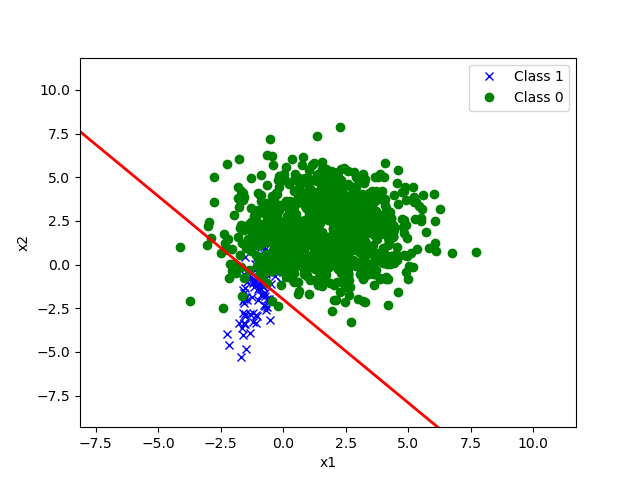
\includegraphics[width=\textwidth]{../src/imbalanced/vanilla.png}
        \caption{Vanilla logistic regression}
        \label{fig:vanilla-sol}
    \end{figure}
\end{answer}
		}\fi

		\item \subquestionpoints{5} \textbf{Re-sampling/Re-weighting Logistic Regression}

The relatively low accuracy for the minority class and the resulting low balanced accuracy are undesirable for many applications. Various methods have been proposed to improve the accuracy for the minority class, and learning imbalanced datasets is  an active open research direction. Here we introduce a simple and classical re-sampling/re-weighting technique that helps improve the balanced accuracy in most of the cases. 

We observe that the logistic regression algorithm works well for the accuracy but not for the balanced accuracy. Let $\mathcal{D} = \{(x^{(i)}, y^{(i)})\}_{i=1}^n$ denote the existing training dataset. We will create a new dataset $\mathcal{D}'$ such that the accuracy on $\mathcal{D}'$ is the same as the balanced accuracy on $\mathcal{D}$.

Assume $\rho < 1/2$ without loss of generality, and let $\kappa = \frac{\rho}{1-\rho}$. This means the number of positive examples is $\kappa$ times the number of negative examples in $\calD$. Assume for convenience $1/\kappa$ is an integer.\footnote{otherwise we can round up to the nearest integer with introducing a slight approximation.} Let $\mathcal{D}'$ be the dataset that contain each negative example once and $1/\kappa$ repetitions of each positive example in $\calD$. Then we will apply the logistic regression on the new dataset $\mathcal{D}'$.  

{\bf Prove that} for any classifier, the balanced accuracy on $\calD$ is equal to the accuracy on $\calD'$. Moreover, {\bf show that} the average empirical loss for logistical regression on the dataset $\calD'$ is equal to 


\begin{align*}
J(\theta) &= -\frac{1+\kappa}{2n} \sum_{i=1}^\nexp w^{(i)} \left(y^{(i)}\log(h_{\theta}(x^{(i)}))
+  (1 - y^{(i)})\log(1 - h_{\theta}(x^{(i)}))\right),
\end{align*}
where $w^{(i)} = 1$ if $y^{(i)} =0$ and $w^{(i)} = 1/\kappa$ if $y^{(i)} = 1$.


Observe effectively we are re-weighting the loss function for each example by some constant that depends on the frequency of the class it belongs to.



		\ifnum\solutions=1 {
		\begin{answer}
\end{answer}
		}\fi

        \item \subquestionpoints{5} \textbf{Coding problem: re-weighting minority class}

In \texttt{src/imbalanced/imbalanced.py}, implement the logistic regression algorithm on $\calD'$.  Compute and report the classifier's accuracy ($A$), balanced accuracy ($\overline{A}$), accuracies for the two classes ($A_0, A_1$) on the validation dataset. You are expected to see that the accuracy of minority class (class 1) improved significantly whereas that of the majority class dropped compared to vanilla logistic regression. However, the balanced accuracy is significantly greater than that of the vanilla logistic regression. 


Create a plot to visualize the validation set with $x_1$ on the horizontal axis and $x_2$ on
the vertical axis. Use different symbols for examples $x^{(i)}$ with true label $y^{(i)} = 1$
than those with $y^{(i)} = 0$. On the same figure, plot the decision boundary obtained
by your model (i.e, line corresponding to model's predicted probability = 0.5) in red color. Include
this plot in your writeup.



        \ifnum\solutions=1 {
        	\begin{answer}
    Classifier's accuracy $A \approx 0.8982$, balanced accuracy $\overline{A} \approx 0.913$.
    Accuracy for two classes $A_0 = 0.895$, $A_1 = 0.93$. These accuracy are computed with code.
    We observed the expected behavior.
    \begin{figure}[H]
        \centering
        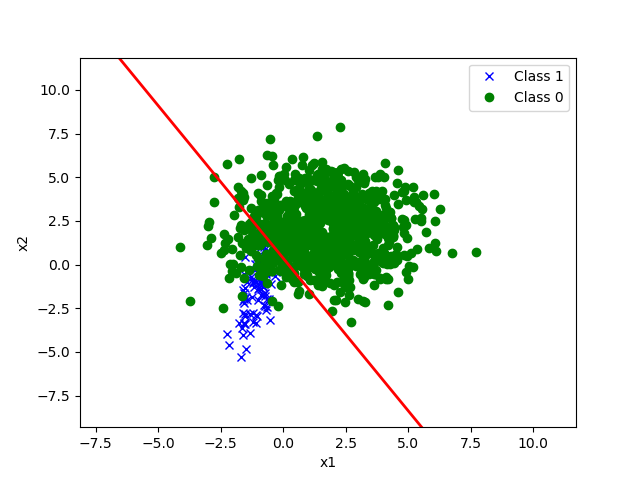
\includegraphics[width=\textwidth]{../src/imbalanced/upsampling.png}
        \caption{Logistic regression with re-sampling and re-weighted loss}
        \label{fig:coding-sol}
    \end{figure}
\end{answer}
        }\fi
   

    
\end{enumerate}
